%%
%% This is file `./samples/longsample.tex',
%% generated with the docstrip utility.
%%
%% The original source files were:
%%
%% apa7.dtx  (with options: `longsample')
%% ----------------------------------------------------------------------
%% 
%% apa7 - A LaTeX class for formatting documents in compliance with the
%% American Psychological Association's Publication Manual, 7th edition
%% 
%% Copyright (C) 2021 by Daniel A. Weiss <daniel.weiss.led at gmail.com>
%% 
%% This work may be distributed and/or modified under the
%% conditions of the LaTeX Project Public License (LPPL), either
%% version 1.3c of this license or (at your option) any later
%% version.  The latest version of this license is in the file:
%% 
%% http://www.latex-project.org/lppl.txt
%% 
%% Users may freely modify these files without permission, as long as the
%% copyright line and this statement are maintained intact.
%% 
%% This work is not endorsed by, affiliated with, or probably even known
%% by, the American Psychological Association.
%% 
%% ----------------------------------------------------------------------
%% 
\documentclass[stu, floatsintext, helv]{apa7}

\usepackage{lipsum}

\usepackage{enumitem}

\usepackage[american]{babel}

\usepackage{tikz}
\usetikzlibrary{shapes.geometric, arrows, positioning, calc}
\usepackage{csquotes}
\usepackage{pdfpages}
\usepackage{float}
\usepackage{caption}
\usepackage{subcaption}
\usepackage{makecell}
\usepackage{placeins}
\usepackage[style=apa,backend=biber]{biblatex}
\addbibresource{bibliography.bib}


\renewcommand\theadalign{cc} % Zentriert den Text in der Kopfzeile
\renewcommand\theadfont{\bfseries} % Fettgedruckter Text für die Kopfzeile
\renewcommand\cellalign{l} % Setzt die Standardausrichtung von makecell auf linksbündig


\title{Gender Differences in the Impact of Gamification Elements on Performance and Anxiety}
\shorttitle{Gender Differences in the Impact of Gamification Elements}

%\authorsnames{Robin Gebert, Nadine Koch, Niklas Meißner, Jun.-Prof. Dr. rer. nat. Maria Wirzberger}
%\authorsaffiliations{University of Stuttgart}
\author{Robin Gebert}
\authorsaffiliations{University of Stuttgart}
\course{Informatik - B.A. (Lehramt)}
\professor{Jun.-Prof. Dr. rer. nat. Maria Wirzberger}
\advisor{Nadine Nicole Koch, M.Sc.\newline\noindent Niklas Meißner, M.Sc.}
\startdate{06. Mai 2024}
\enddate{06. September 2024}

\leftheader{Gebert}

\abstractGerman{Diese Bachelorarbeit untersucht die Auswirkungen verschiedener Gamification-Elemente auf Leistung und Angst in digitalen Lernumgebungen, mit einem besonderen Fokus auf Geschlechterunterschiede. Trotz der breiten Anwendung von Gamification in Bildungstechnologien ist das Verständnis darüber, wie individuelle Faktoren wie Geschlecht diese Effekte beeinflussen, begrenzt. Die Studie verwendet ein 2$\times$8 faktorielles Design, um die Interaktionen zwischen Gamification-Elementen und Geschlecht zu analysieren, wobei 117 Teilnehmer aus verschiedenen Studiengängen rekrutiert wurden. Die Ergebnisse zeigen, dass verschiedene Gamification-Elemente die Leistung und Angst unterschiedlich beeinflussen, jedoch waren diese Gruppenunterschiede überwiegend deskriptiv und nicht signifikant. Diese Erkenntnisse deuten darauf hin, dass die Anpassung von Gamification-Strategien an geschlechtsspezifische Reaktionen potenziell die Effektivität von digitalen Lernumgebungen verbessern könnte. Die Studie betont die Notwendigkeit weiterer Forschungen, um die Beziehung zwischen Gamification, Geschlecht und Lernausgängen tiefer zu verstehen.}
\keywordsGerman{Gamification, Geschlecht, Intelligente Tutorielle Systeme, Leistung, Angst}

\abstractEnglish{This bachelor thesis explores the effects of various gamification elements on performance and anxiety in digital learning environments, with a specific focus on gender differences. Despite the widespread application of gamification in educational technologies, understanding of how individual factors such as gender influence these effects remains limited. The study employed a 2$\times$8 factorial design to analyze interactions between gamification elements and gender, recruiting 117 participants from various degree programs. Findings indicate that different gamification elements variably affect performance and anxiety, however, these group differences were predominantly descriptive and not significant effects. These insights suggest that tailoring gamification strategies to gender-specific responses could potentially enhance the effectiveness of digital learning environments. The study underscores the need for further research to deepen understanding of the relationship between gamification, gender, and learning outcomes.}
\keywordsEnglish{Gamification, Gender, Intelligent tutoring systems, Performance, Anxiety}

%%
%%\authornote{
%%   \addORCIDlink{Daniel A. Weiss}{0000-0000-0000-0000}
%%
%%  Correspondence concerning this article should be addressed to Daniel A. Weiss, Department of Educational Psychology, Counseling and
%%  Special Education, A University Somewhere, 123 Main St., Oneonta, NY
%%  13820.  E-mail: daniel.weiss.led@gmail.com}
%%
\begin{document}
\maketitle


%% !TeX spellcheck = en_US
Gamification, especially in the context of education is nothing new and has been used by societies long before the modern era.
The concept of grading can be seen as a form of gamification, as it adds feedback and a competitive element to the learning process.
But in recent years especially with the advance of computers, gamification has become an increasingly popular topic in education science \parencite{swachaStateResearchGamification2021}.
Especially in computer science the use of gamified elements is well researched \parencite{dichevGamifyingEducationWhat2017}, which could be related to the already great use of computers in the field.
But as the topic is still relatively new and many topics are still not well researched.

\section{Introduction}
one paragraph per item of the abstract. However, provide more details and do not just copy sentences from the abstract. 
Additionally, provide  another paragraph and  Make your own \textbf{contribution(s)} explicit ("The contribution of this thesis is...").


\subsection*{Thesis Structure}
Here, give an overview of your thesis structure.
\begin{description}
\item[Section~\ref{chap:evaluation} -- \nameref{chap:evaluation}:] Here, we provide...
\item[Section~\ref{chap:conclusion} -- \nameref{chap:conclusion}] We conclude our thesis ...
\end{description}

\section{Theoretical Background}

\subsection{Gamified digital learning environments}
Digital learning environments
Intelligent Tutoring Systems (ITS) can be referred to as "any computer program that can be used in learning and that contains intelligence" \>\parencite{freedmanLinksWhatIntelligent2000}.
Therefore, ITS accompany a student on his or her learning experience of a specific domain of knowledge by creating tasks that appeal to the students needs \parencite{gonzalezGamificationIntelligentTutoring2014}.
ITS can range from simple instructive texts to simulations and virtual realities, as a model imitating and abstracting certain aspects of the real world to reduce complexity for machine and user \parencite{psotkaIntelligentTutoringSystems1988}.
Modern ITS are split into three intertwined models: student, domain and tutor model. The student model holds the information about the user.
The user is characterized from different angles the information is updated as the user advances within the ITS.
The domain model contains the knowledge and structure of the learning material. It supplies the tutor model with tasks based on the input from the student model.
At last the tutor model controls the interaction with the student and contains the information which tasks are shown to the user in accord with the learning objectives from the domain model (\cite{gonzalezGamificationIntelligentTutoring2014}; \cite{freedmanLinksWhatIntelligent2000}).

With the rising interest in Gamification ITS also grow in importance as they can be used together. The use of gamified elements enhances the ITS and Gamification require some sort of progress tracking model for the gamified elements (e.g. Content unlocking to work).
\Textcite{gonzalezGamificationIntelligentTutoring2014} suggest adding more models as Gamification requires additional systems for visualization and feedback.
Additionally, new studies created a connection between emotions and learning, other studies connected relationships between teachers and students and an increase in student motivation \parencite{woolfAffectiveTutorsAutomatic2010}.
Both results were linked in a study by \Textcite{woolfAffectiveTutorsAutomatic2010} showing how digital learning companions improved the overall learning ability and self-concept of all students, especially low achieving students.
For the context of this thesis it is also important that the ITS version with a male learning companion was muted twice as much as the female version, resulting in a lower effect.
The study showed differences between gender, in discussion \Textcite{woolfAffectiveTutorsAutomatic2010} suggested considering gender within the student domain could further advance its predictive power.


\subsection{Gamification}
Gamification can be defined as "the idea of using game design elements in non-game contexts" \>\parencite{deterdingGameDesignElements2011} to further increase motivation and user activity within interaction design \parencite{deterdingGameDesignElements2011}.
These game-design elements "gamified elements" are elements often found in classical games. Often used elements are points, badges, leaderboards and avatars, other mechanisms include content unlocking, storytelling and memes \parencite{zainuddinImpactGamificationLearning2020}.
Often those elements are used specific constellations like the PBL triad described by \cite{werbachWinHowGame2012}, which contains points, badges and leaderboards, a system that is not only known from games, but also everyday enterprise features like loyalty programs and employee competitions \parencite{werbachWinHowGame2012}.
Points because they add an absolute scale, badges because they represent a status symbol and work like a temporary goal to strive toward and leaderboards to compare yourself to peers \parencite{werbachWinHowGame2012}.
One of the positive effects of gamification is brought by the feedback in different forms (task, process, self-regulation, self) either immediate or delayed. Feedback is one of the most important factors in the relation between education and learning \cite{sailerGamificationLearningMetaanalysis2020}.
The use of gamified elements showed positive outcomes in multiple studies, in general \parencite{hamariDoesGamificationWork2014} as well as in education specific contexts \parencite{sailerGamificationLearningMetaanalysis2020}.
But gamification, especially some elements like leaderboards, can also lead to negative outcomes. Leaderboards, while motivating through comparison, have been reported to demotivate participants \parencite{almeidaSystematicMappingNegative2021}.
"Pavlovication" as \cite{klabbersArchitectureGameScience2018} calls it, Gamification, as it is often a short question-answer-reward-cycle, conditions the user to learn conditional and narrows the possible ways to solve a problem down ~\parencite{klabbersArchitectureGameScience2018}.
Some studies also suggested that gamified learning platforms also lack individualism regarding choice and display of gamification elements, resulting in discomfort and negative emotions \parencite{santosDoesGenderStereotype2023}.

\subsection{Gender and Stereotype threat}
Gender, as a concept within social sciences, refers to more than the binary categorization of male and female.
It encompasses a range of identities and experiences that are shaped by a complex interplay of biological, psychological, and social factors.
Gender is not solely determined by biological characteristics; instead, it is increasingly recognized as a spectrum, acknowledging the presence of diverse gender identities beyond the traditional binary understanding \parencite{lindqvistWhatGenderAnyway2021}.
Socialization plays a critical role in shaping gender identity. It influences how individuals perceive themselves and interact with their surroundings based on the gender norms prevalent within their society.
These norms dictate behaviors, roles, and expectations, which are often internalized from an early age through various socialization agents like family, media, educational institutions, and peer groups \parencite{kampshoffHandbuchGeschlechterforschungUnd2012}.
While acknowledging the spectrum of gender identities, this thesis will focus primarily on the binary categorization of gender—male and female.
This approach does not negate the validity of non-binary or genderqueer identities but rather limits the scope of investigation to traditional gender roles within the binary framework.

Stereotype threat occurs when "one can be judged by, treated in terms of, or self-fulfill negative stereotypes about one's group".
Although this study does not aim to eliminate stereotype threat it is an important factor as it can explain at least some of the differences different genders experience while studying computer science \parencite{cheryanClassroomsMatterDesign2011}, especially regarding math \parencite{spencerStereotypeThreatWomen1999}.
Stereotype threat even leads to lower identification with academics and specific subjects \parencite{christyLeaderboardsVirtualClassroom2014}.
\section{Hypotheses}

Wie in dem ersten Kapitel zu erkennen, gibt es offene Fragen zu der Effizienz verschiedener gamifizierter Elemente und dem Bezug verschiedener Geschlechter zu diesen gamifizierten Elementen.
Generell ist die Frage nach der Effizienz bestimmter Elemente und Elementkombinationen noch zu klären \parencite{dehghanzadehUsingGamificationSupport2024}.
Um die Verbindung von Geschlecht und Gamification-Elementen zu untersuchen, haben wir folgendes Modell erstellt:
**Modell einfügen**

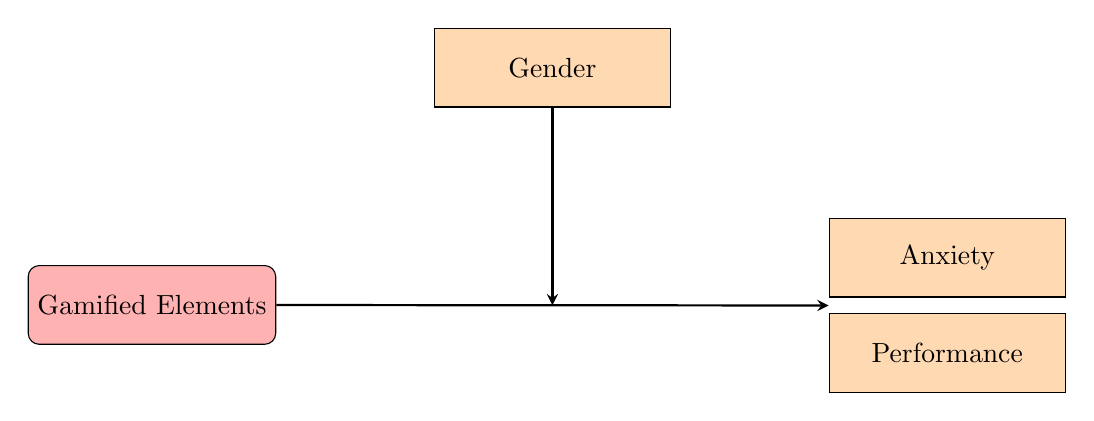
\begin{tikzpicture}[node distance=0cm]
    \tikzstyle{startstop} = [rectangle, rounded corners, minimum width=3cm, minimum height=1cm,text centered, draw=black, fill=red!30]
    \tikzstyle{process} = [rectangle, minimum width=3cm, minimum height=1cm, text centered, draw=black, fill=orange!30]
    \tikzstyle{arrow} = [thick,->,>=stealth]

    \node (gender) [process] {Gender};
    \node (gamified) [startstop, below left=2cm and 2cm of gender] {Gamified Elements};
    \node (anxiety) [process, below right=1.4cm and 2cm of gender] {Anxiety};
    \node (performance) [process, below=0.2cm of anxiety] {Performance};

    \coordinate (MidPoint1) at ($(anxiety.west)!0.5!(performance.west)$);

    % Calculate midpoint for the horizontal arrow
    \coordinate (MidPoint2) at ($(gamified.east)!0.5!(MidPoint1)$);

    \draw [arrow] (gamified) -- (MidPoint1);
    \draw [arrow] (gender) -- (MidPoint2);
\end{tikzpicture}
\section{Methods}
\subsection{Participants}
\subsection{Design}
This study explored the impact of various gamified elements and participant gender on performance and anxiety.
The independent variables were gamified elements, with participants randomly assigned to one of eight conditions: Avatars (A), Badges (B), Points (P), Leaderboards (L), Narrated Content (N), combinations of Points, Badges, Leaderboards, and Avatars (PBLA), Points, Badges, Leaderboards, Avatars, and Narrated Content (PBLAN), and a control group with no gamified elements.
Each participant experienced three distinct conditions, which were sent by the server out of a randomized pregenerated batch, ensuring that all conditions were evenly distributed across participants.
Participants underwent a series of tests in a fixed order during each round, beginning with a gamified performance test in an digital learning environment followed by  not gamified assessments for anxiety, self-efficacy, and motivation.
At the end participants were given a monetary compensation of 15€.
The performance tests utilized standard progressive matrices , adapted with gamification techniques to engage and challenge participants uniquely in each round.
The dependent variables included:
\begin{itemize}
  \item \textbf{Performance}, assessed through accuracy and response times in the gamified progressive matrices.
  \item \textbf{Anxiety}, evaluated using a standardized questionnaire immediately after the performance test. Anxiety was measured using a shortened form of the State-Trait Anxiety Inventory (STAI) with 6 items \parencite{marteauDevelopmentSixitemShortform1992}.
\end{itemize}

Although self-efficacy and motivation were also assessed \parencite{chenValidationNewGeneral2001,guayAssessmentSituationalIntrinsic2000} through subsequent questionnaires, these variables were not analyzed within the scope of this bachelor thesis.
The collected data for self-efficacy and motivation are intended for use in the doctoral dissertation of \textbf{Nadine Koch}.
This research employed a repeated-measures design, where each participant was exposed to three different gamification conditions chosen randomly.
This within-subjects approach facilitated the analysis of individual responses to each condition across the different rounds, providing insights into how variations in gamification can affect psychological states and performance.
The sequence and consistency of the testing procedure, including the series of questions asked in the gamified digital learning environment were always maintained to ensure the reliability of measurements and comparability of results across the various stages of the experiment.


\subsection{Materials}
\subsubsection{Physical environment}
The study was conducted in two seperate rooms in the cellar of a university building, one equipped with five and one with seven iMac's.
As \textcite{christyLeaderboardsVirtualClassroom2014} suggested that the physical environment can influence the results, so both rooms are equipped with the same furniture and lighting and are furnished very dry, like a typical software laboratory.

\subsection{Virtual environment}
The software used in this study was build by the author using SvelteKit in frontend and Ktor in backend. It's UI is designed after the study by \textcite{albuquerqueDoesGenderStereotype2017}.
On the iMac's the study was displayed full-screen mode using the Safari web browser to ensure no further distractions. The study consisted of 4 screens.
A consent screen to give an overview and explain the data collection to the user.
A personal detail screen to collect said data; gender, age and study program. Participants also had to enter a deletion code in order to request their data's deletion after the collection.
\begin{minipage}{\textwidth}
  \includegraphics[width=0.6\textwidth]{img/details.png}
  \captionof{figure}{The personal detail collection form}
  \label{fig:figureDetails}
\end{minipage}
The next screen was the gamified learning environment, where the participants had to solve 20 questions in a row while being exposed to the gamified elements.
The matrices were taken from \textcite{albuquerqueDoesGenderStereotype2017}, to generate 60 questions out of the 20, the 40 questions for iteration two and three were slightly altered versions of the original 20 made by this author.
\begin{minipage}{\textwidth}
  \includegraphics[width=0.6\textwidth]{img/q-17.png}
  \captionof{figure}{A standard progressive matrix, one of the tasks given to the participants}
  \label{fig:figureMatrix}
\end{minipage}
The gamified learning environment consists of different UI elements representing the gamified elements.
\begin{description}
  \item[Leaderboards]: A list of participants and scores, including the current participant. The other players shown are not real.
  \item[Badges]: An array of four badges that are awarded for 1, 5, 10 and 18 correctly answered questions.
  \item[Avatars]: A small avatar that is shown in the top right corner of the screen and on the leaderboard. To increase identification with the avatar further, the participants were asked to choose one of 15 different avatars before the iteration.
  \item[Narrated content]: Narrated content is shown in the bottom right corner of the screen. It is presented as a speech bubble with an avatar next to it, in case avatars are enabled. It shows a random praise or encouragement sentence every three questions.
  \item[Points]: A counter next to the question frame shows the current points. One point is awarded for each correctly answered question. THe narrated content is shown every three questions.
\end{description}
After answering one question the next question has a 1 second delay which increases to 4 seconds if narrated content is shown.
\begin{minipage}{\textwidth}
  \includegraphics[width=0.3\textwidth]{img/question_screen.png}
  \captionof{figure}{The Digital Learning Environment with Points, Badges, Leaderboards and Avatars enabled.}
  \label{fig:figureScreen}
\end{minipage}
\begin{minipage}{\textwidth}
  \includegraphics[width=0.3\textwidth]{img/question_screen_no_elements.png}
  \captionof{figure}{The Digital Learning Environment with Points, Badges, Leaderboards and Avatars enabled.}
  \label{fig:figureScreen}
\end{minipage}
After the gamified learning environment, the participants were shown a questionnaire for anxiety, motivation and self-efficacy. The three questionnaires were a six-question shortened form of the State-Trait Anxiety Inventory (STAI) \parencite{marteauDevelopmentSixitemShortform1992}, the eight-question General Self-Efficacy Scale (GSE) \parencite{guayAssessmentSituationalIntrinsic2000} and the 16-question Situational Intrinsic Motivation Scale (SIMS) \parencite{chenValidationNewGeneral2001}.



\subsection{Procedure and Materials}
The study was conducted in two seperate rooms, one equipped with five and one with seven iMac's. The study was displayed in full-screen mode to ensure no further distractions.
At the start participants were shown a consent form as at least some personal data was collected, namely gender, age and study program. Participants also had to enter a deletion code in order to request their data's deletion after the collection.
\begin{minipage}{\textwidth}
  \includegraphics[width=0.6\textwidth]{img/details.png}
  \captionof{figure}{The personal detail collection form}
  \label{fig:figureDetails}
\end{minipage}
Afterwards the study proceeded to three iterations of 20 questions each, that are based on Progressive Matrices used by \Textcite{albuquerqueDoesGenderStereotype2017}.
Every iteration was followed by three questionnaires for anxiety, motivation and self-efficacy. Then a data submission dialog guided the participants to the next iteration.
\subsubsection{Question items}
\begin{minipage}{\textwidth}
  \includegraphics[width=0.6\textwidth]{img/q-17.png}
  \captionof{figure}{A standard progressive matrix, one of the tasks given to the participants}
  \label{fig:figureMatrix}
\end{minipage}
To generate 60 questions out of the 20 from\textcite{albuquerqueDoesGenderStereotype2017}, the questions were slightly altered by this author.
These questions are embedded into the digital gamified learning environment.
\subsubsection{Gamified Digital Learning Environment}
The Environment used a combination of different Gamified Elements for each iteration.
\begin{minipage}{\textwidth}
  \centering
  \includegraphics[width=0.6\textwidth]{img/question_screen.png}
  \captionof{figure}{The Digital Learning Environment with Points, Badges, Leaderboards and Avatars enabled.}
  \label{fig:figureScreen}
\end{minipage}

\subsection{Scoring}
% !TeX spellcheck = en_US

\section{Results}
\label{chap:evaluation}
\subsection{Data Exclusion}
Participants who identified their gender as "other" were excluded from the analysis because the present research available and used for this thesis primarily focuses on comparisons between male and female participants.
This criterion led to the exclusion of two participants. Additionally, participants who achieved less than 25\% correct answers in the gamified learning environment were excluded.
This threshold was set because there were five possible answers for each question, and random clicking would statistically result in a 20\% correct response rate.
Therefore, a performance below 25\% suggests either random guessing or a fundamental misunderstanding of the task.
Furthermore, any incomplete data sets were excluded to ensure the integrity and consistency of the analysis, resulting in the exclusion of one additional participant.
Initially, there were 120 data sets, and after applying the exclusion criteria, 117 data sets remained.

\subsection{Outline of Statistical Analysis}
Having preprocessed and cleaned the data, we proceeded with our statistical analysis using linear mixed models (LMMs).
These models were chosen for their ability to handle the complexities of repeated measures from the same subjects under varying conditions.
By incorporating both fixed effects (gender and gamified elements) and random effects (individual differences), LMMs provided a robust framework for our analysis.

We utilized the Nelder-Mead optimization method to estimate the parameters of our models.
This method is ideal for our needs as it efficiently handles models with multiple interacting effects without requiring derivative calculations, making it suitable for our complex dataset.

For the estimation of variance components within our models, we employed Restricted Maximum Likelihood (REML).
REML is preferred in mixed model contexts because it adjusts the estimates for the fixed effects, providing unbiased variance estimates despite the presence of random effects.

Finally, to ensure accurate inference regarding the fixed effects, we applied the Satterthwaite approximation for estimating degrees of freedom.
This method helps in achieving more reliable p-values by adjusting the degrees of freedom for the complexity of the model, crucial in cases with multiple levels of interactions and a limited sample size.

This combination of methods and their implementation through LMMs allowed us to systematically analyse the effects of gender and gamified elements on performance and anxiety, controlling for individual variability and the specifics of the experimental design.

\subsection{Report of findings}

\subsubsection{Performance}
Women exhibited lower performance levels when leaderboards were the gamified element used (\textit{M}= .700, \textit{SE} = .056) compared to men (\textit{M} = .835, \textit{SE} = .024) and to the overall average performance in gamified settings for women (\textit{M} = .846, \textit{SE} = 0.030).
Notable is also the variability suggested by the large standard error for women in this leaderboard condition.
Despite some descriptive effects, our analysis revealed no significant main effects or interactions for all hypotheses regarding performance, as documented in \autoref{tab:lmm_performance}.

\begin{figure}[h]
    \centering
    \begin{subfigure}[b]{0.45\textwidth}
        \includegraphics[width=\textwidth]{img/plots/grey/plot_performance.png}
        \label{fig:plot_performance}
    \end{subfigure}
    \hfill
    \begin{subfigure}[b]{0.45\textwidth}
        \includegraphics[width=\textwidth]{img/plots/grey/plot_performance_gender.png}
        \label{fig:plot_performance_gender}
    \end{subfigure}
    \caption{On the left: Overall performance across different gamification elements as percentage. On the right: Performance by gender grouped by gamification element as percentage.}
    \label{fig:performance_comparison}
\end{figure}

\begin{table}[h]
    \centering
    \caption{Results of the linear mixed model analysis for percentage correct effects.}
    \label{tab:lmm_performance}
    \begin{tabular}{lcccc}
        \hline
        Variable & \textit{beta} & \textit{p} & \textit{t} & \textit{df} \\
        \hline
        m & 0.07 & .994 & 0.27 & 277.62 \\
        P & -0.33 & .493 & -1.35 & 211.82 \\
        B & 0.06 & .994 & 0.21 & 214.27 \\
        L & -0.48 & .384 & -1.67 & 213.69 \\
        A & 0.13 & .994 & 0.49 & 208.19 \\
        N & 0.44 & .384 & 1.70 & 207.03 \\
        PBLA & 0.01 & .994 & 0.06 & 208.37 \\
        PBLAN & 0.06 & .994 & 0.22 & 210.22 \\
        m $\times$ P & 0.42 & .493 & 1.33 & 214.33 \\
        m $\times$ B & -0.22 & .994 & -0.64 & 213.78 \\
        m $\times$ L & 0.61 & .384 & 1.79 & 214.82 \\
        m $\times$ A & 0.01 & .994 & 0.03 & 209.52 \\
        m $\times$ N & -0.00 & .994 & -0.01 & 210.19 \\
        m $\times$ PBLA & 0.37 & .548 & 1.18 & 211.59 \\
        m $\times$ PBLAN & 0.01 & .994 & 0.02 & 210.43 \\
        \hline
    \end{tabular}
    \tablenote{Abbreviations: m = Male, P = Points, B = Badges, L = Level, A = Avatars, N = Narrative Content, PBLA = Combination of Points, Badges, Level, and Avatars, PBLAN = Combination of all elements. Male is compared to female performance, gamified elements are compared to the non-gamified environment. The interactions are compared to female in the non-gamified environment.}
\end{table}




\subsubsection{Anxiety}
Some descriptive trends emerged from our analysis, as illustrated in \autoref{fig:anxiety_comparison}.
Women experienced higher anxiety levels than men in the non-gamified environment (\textit{M} = .571, \textit{SE} = .092 for women compared to \textit{M} = .296, \textit{SE} = .099 for men) and when leaderboards were used (\textit{M} = .683, \textit{SE} = .205 for women compared to \textit{M} = .566, \textit{SE} = .119 for men).
In contrast, the use of avatars was associated with lower anxiety levels for women (\textit{M} = .187, \textit{SE} = .095) than for men (\textit{M} = .476, \textit{SE} = .102).

Despite these trends, our analysis revealed no significant main effects or interactions for any of the hypotheses regarding anxiety levels, as detailed in \autoref{tab:lmm_stai}.
This leads us to conclude that the hypotheses regarding anxiety must be rejected.


\begin{figure}[h]
    \centering
    \begin{subfigure}[b]{0.45\textwidth}
        \includegraphics[width=\textwidth]{img/plots/grey/plot_anxiety.png}
    \end{subfigure}
    \hfill
    \begin{subfigure}[b]{0.45\textwidth}
        \includegraphics[width=\textwidth]{img/plots/grey/plot_anxiety_gender.png}
    \end{subfigure}
    \caption{On the left: Anxiety levels across different gamification elements. On the right: Differences in anxiety levels by gender grouped by gamified element.}
    \label{fig:anxiety_comparison}
\end{figure}

\begin{table}[h]
    \centering
    \caption{Results of the linear mixed model analysis for STAI effects.}
    \label{tab:lmm_stai}
    \begin{tabular}{lccccc}
        \hline
        Variable & \textit{beta} & \textit{p} & \textit{t} & \textit{df} \\
        \hline
        m & -0.25 & .623 & -0.83 & 288.25 \\
        P & -0.28 & .564 & -1.00 & 216.76 \\
        B & 0.23 & .623 & 0.73 & 221.07 \\
        L & -0.04 & .913 & -0.11 & 220.38 \\
        A & -0.62 & .228 & -2.11 & 213.37 \\
        N & -0.53 & .241 & -1.81 & 211.70 \\
        PBLA & -0.03 & .913 & -0.11 & 213.53 \\
        PBLAN & -0.60 & .228 & -2.04 & 215.77 \\
        m $\times$ P & 0.42 & .481 & 1.18 & 220.20 \\
        m $\times$ B & -0.18 & .787 & -0.47 & 220.26 \\
        m $\times$ L & 0.28 & .623 & 0.74 & 221.54 \\
        m $\times$ A & 0.64 & .241 & 1.79 & 214.84 \\
        m $\times$ N & 0.50 & .437 & 1.40 & 215.47 \\
        m $\times$ PBLA & 0.10 & .882 & 0.29 & 217.43 \\
        m $\times$ PBLAN & 0.45 & .481 & 1.25 & 215.91 \\
        \hline
    \end{tabular}
    \tablenote{Abbreviations: m = Male, P = Points, B = Badges, L = Leaderboards, A = Avatars, N = Narrative Content, PBLA = Combination of Points, Badges, Leaderboards, and Avatars, PBLAN = Combination of all elements. Male is compared to female anxiety, gamified elements are compared to the non-gamified environment. The interactions are compared to female in the non-gamified environment.}
\end{table}
\section{Discussion}
%\subsection{Summary of Research focus}
In recent years gamification has gained popularity as a tool to enhance learner performance in various domains, including education.
However, the effects of gamification elements on different groups, particularly in digital learning environments, remain underexplored.
This thesis explored the effects of gamification elements on performance and anxiety in digital learning environments, with a focus on gender differences.
Using a randomized controlled design, the study assessed various gamification components like points, badges, leaderboards, and avatars, analysing responses from male and female participants.
The main goal was to identify how different genders react to these gamified elements regarding their cognitive and affective states.

Although the study did not find statistically significant effects, the results obtained were in line with existing research previously mentioned, indicating consistent patterns in how participants especially of different gender reacted to the gamification elements.
This suggests that while the group differences were not strong enough to be statistically significant, the observed behaviours reflected known theories and previous studies.

\subsection{Interpretation}
This study's findings did not reveal statistically significant effects but group differences, suggesting that gamification impacts might be subtle and context-specific.
These results align with prior research \parencite{hamariDoesGamificationWork2014}, which also reported variable impacts of gamification on learning.
The study underscores the need for cautious interpretation given the complexity of gamification's effects on different learners.

%These observed trends align with previous research that also noted similar patterns without definitive effects \parencite{dehghanzadehUsingGamificationSupport2024,hamariDoesGamificationWork2014}.
%While the absence of the expected effect is noteworthy, it does not necessarily indicate that the effect does not exist.
%For example maybe the estimated effect sizes are smaller than assumed and hence there were to less participants per condition to find these differences.
%It's worth considering that the effect might be inherently more complex or context-dependent than originally hypothesized as also indicated by \textcite{dehghanzadehUsingGamificationSupport2024,koivistoRiseMotivationalInformation2019,oliveiraTailoredGamificationEducation2023}.
%The failure to detect the effect might suggest that it only emerges under certain conditions or within particular subgroups, which our study design did not fully capture.
%Additionally, the group of participants seems to be very homogenous, as the majority of students were bachelor students recruited from the computer science building.


\subsection{Implications}
The absence of statistically significant effects in this study does not allow for definitive conclusions regarding the impact of gamification on learning outcomes.
This result challenges the theoretical assumptions laid out early in this thesis, suggesting a more complex interaction between gamification and learner engagement that is likely dependent on contextual and individual differences.
The observed group differences, although not significant, hint at the variability in how learners respond to gamified elements. 

From a practical perspective, the non-significant findings although not suggesting specific solutions imply that the one-size-fits-all approach to gamification may not be effective for all learners.
Educational software designers might consider developing more adaptive gamification strategies that are tailored to the educational and personal context of their learners.
Such customization could enhance the effectiveness of educational interventions by aligning more closely with the diverse needs of students.
As mentioned, without significant effects this study suggests the potential benefits of continuous adaptation and testing of gamification strategies in educational settings.
Future research should aim to explore and validate these strategies as also suggested by \textcite{dehghanzadehUsingGamificationSupport2024,koivistoRiseMotivationalInformation2019,oliveiraTailoredGamificationEducation2023}, but also consider the limitations this study showed.


%\subsection{Implications}
%Theoretically, the observed trends, hint at potential variations in how gamification impacts different learners, suggesting a need for more fine grained systems.
%This could inspire further research into personalized learning environments.
%Practically, these preliminary findings encourage a cautious approach to integrating gamification in educational settings.
%Designers might consider more flexible gamification systems that can be adjusted based on gender, potentially enhancing user engagement without a one-size-fits-all strategy.
%An example would be to implement leaderboards in male classes and use of avatars in female classes.


\subsection{Limitations}
This study has several key limitations that must be acknowledged.
Firstly, the reliance on self-reported data from students may lead to potential biases and inaccuracies in the findings. Previous research suggests that objective measures, such as sensor-based tracking, could provide more reliable data \parencite{woolfAffectiveTutorsAutomatic2010}.

Another significant limitation arises from the demographic and location constraints of our sample. The majority of participants were recruited from the computer science learning room, where officially only computer science students have access. This building is on the technical campus, which may not provide a diverse representation of the general student population.

Additionally, the customization options for avatars were limited, lacking diverse representations such as Hijabs or beards, as noted by participants. This limitation may affect the engagement and identification of users with the avatars. It would have also been beneficial to allow users to personalize their avatars by entering their names, as this could further enhance user engagement and identification with the avatar.

The narrated content of the gamified elements could also be not engaging enough, being confined to a small portion of the screen without integrating characteristics, abilities, or additional dialogues that could enhance user interaction, while consuming additional time until the user could proceed. This might have contributed to some participants recalling to ignore the gamified elements altogether, thus not experiencing the intended gamified environment fully.
Furthermore, the design of the study involved three iterations per participant, which might have led to habituation effects. These effects could influence the outcomes in terms of learning environment adaptability, anxiety, motivation, and self-efficacy, thus potentially diminishing the study's ability to measure these constructs accurately over time.

Finally, the lack of sufficient individualized feedback by the participants post-study was highlighted as a concern. Future studies should consider incorporating mechanisms for feedback. This could provide valuable insights into the participants' experiences and perceptions of the gamified elements, potentially revealing more nuanced effects that were not captured in this study.
Despite these limitations, the findings provide valuable insights into the intersection of gamification and gender, suggesting avenues for future research and practical applications in educational environments.
\newpage
\subsection{Future Research}
As highlighted in the introduction, the exploration of individual characteristics in the selection of gamified elements within learning environments requires further investigation.
This thesis has laid foundational insights into how gender influences engagement with gamified systems. 
However based on our results, the gamified elements showing descriptive trends, especially leaderboards and avatars in this study should be further explored.
For example, different leaderboard styles with varying avatar integrations could be tested in order to mitigate gender differences.
As badges seem to have a negative outcome on anxiety, further research could explore the use of avatars in various implementations to counteract this effect for female students.
Other dimensions such as age, culture, and notably, the educational level (ranging from school-level to higher education and adult learning) merit in-depth exploration to comprehensively understand the dynamics at play.

Moreover, while the study's learning environment provided a basic platform, it does not directly represent the probable application of gamified elements. As ITS focus on supporting the learning process through building a model for teaching in the style best suited for the individual, future studies should implement some sort of intelligence, not only in gamified elements but also the learning content shown to the student.

Additionally, the temporal scope of this study was limited, addressing only short-term interactions. Prior research has established the significance of longitudinal studies in this domain \parencite{oliveiraTailoredGamificationEducation2023,dehghanzadehUsingGamificationSupport2024}. Extending research timelines to span multiple semesters would provide a more robust understanding of the long-term impacts of gamification on learning outcomes and student engagement. Such extended studies are quite challenging in every research area, but crucial for observing changes in learner stategies and behaviour and the sustainability of gamification benefits over time.

In conclusion, advancing research in these areas will not only enrich our understanding of how different groups respond to gamified learning but also enhance the design and implementation of educational technologies that are inclusive and effective across diverse learning environments.

\subsection*{Conclusion}
This study's exploration into the effects of gamification elements on performance and anxiety with a focus on gender differences has provided initial insights that, while not statistically significant, point to subtle yet potentially important trends.
The observed data suggest that certain gamified elements could have differential impacts on cognitive and affective outcomes across genders.
Although these effects were not strong enough to achieve statistical significance in this study, the descriptive findings hint at underlying patterns that merit further investigation.

The consistency of these patterns with prior research indicates that with improved research designs that address the limitations of this study, significant findings could be obtained.
These findings could be very important for advancing the understanding of how gamification can be optimized to enhance performance and anxiety effectively.
Future research should consider these aspects to uncover more robust evidence that can contribute to the ongoing discourse in educational technology.


\subsection*{Acknowledgements}
We acknowledge the support of the German Research Foundation (DFG; DFG reference number UP 31/1) for funding the Stuttgart Research Focus Interchange Forum for Reflecting on Intelligent Systems (IRIS).
This research was further supported by the Ministry of Science, Research, and the Arts (MWK) Baden-Württemberg, Germany, within the Artificial Intelligence Software Academy (AISA; reference number Az. 7542.2-9-47.10/36/2).

\printbibliography

\end{document}

%% 
%% Copyright (C) 2021 by Daniel A. Weiss <daniel.weiss.led at gmail.com>
%% 
%% This work may be distributed and/or modified under the
%% conditions of the LaTeX Project Public License (LPPL), either
%% version 1.3c of this license or (at your option) any later
%% version.  The latest version of this license is in the file:
%% 
%% http://www.latex-project.org/lppl.txt
%% 
%% Users may freely modify these files without permission, as long as the
%% copyright line and this statement are maintained intact.
%% 
%% This work is not endorsed by, affiliated with, or probably even known
%% by, the American Psychological Association.
%% 
%% 
%% This work is "maintained" (as per LPPL maintenance status) by
%% Daniel A. Weiss.
%% 
%% This work consists of the file  apa7.dtx
%% and the derived files           apa7.ins,
%%                                 apa7.cls,
%%                                 apa7.pdf,
%%                                 README,
%%                                 APA7american.txt,
%%                                 APA7british.txt,
%%                                 APA7dutch.txt,
%%                                 APA7english.txt,
%%                                 APA7french.txt,
%%                                 APA7german.txt,
%%                                 APA7ngerman.txt,
%%                                 APA7greek.txt,
%%                                 APA7czech.txt,
%%                                 APA7turkish.txt,
%%                                 APA7endfloat.cfg,
%%                                 Figure1.pdf,
%%                                 shortsample.tex,
%%                                 longsample.tex, and
%%                                 bibliography.bib.
%% 
%%
%% End of file `./samples/longsample.tex'.